\documentclass[12pt]{article}

% preamble
\usepackage{amsmath}
\usepackage[margin = 1in]{geometry}
\usepackage{graphicx}
\usepackage{booktabs}
\usepackage{natbib}

% highlighting hyper links
\usepackage[colorlinks=true, citecolor=blue]{hyperref}

\title{Comparison of Multi-Class Classification Methods}
\author{Sean Murphy\\
  Statistics Major\\
  University of Connecticut
}

\begin{document}
\maketitle

\begin{abstract}
THE ABSTRACT WILL BE WRITTEN AFTER THE REST OF THE PAPER HAS BEEN WRITTEN. 
\end{abstract}

\section{Introduction}
\label{sec:intro}

% Use this section to answer three questions:
% Why is the topic important/interesting?
% What has been done on this topic in the literature?
% What is your contribution?

The rest of the paper will be organized in the following way.  
An introduction to the red wine data set will be presented in 
Section~\ref{sec:data}.  This section will describe the variables 
and observations contained in the dataset, and will include a brief 
overview of summary statistics.  Next, a methodological overview of 
this analysis will be given in Section~\ref{sec:meth}.  Each of the 
classification methods and their underlying assumptions will be 
presented in Section~\ref{sec:class}.  The classification metrics 
which will be used to compare the predictive effectiveness of each 
model will be introduced in Section~\ref{sec:metr}.  After this, 
the results will be presented with tables and figures in 
Section~\ref{sec:resu}.  Finally, once the results of the analysis 
have been described, a discussion of their implications and 
suggestions for further study will be covered in Section~\ref{sec:disc}.


\section{Data}
\label{sec:data}

The data that will be analyzed in this study comes from the UC Irvine Machine 
Learning Repository.  It is a dataset from 2009 containing information about 
a sample of red "Vinho Verde" wine from north Portugal.  The dataset contains 
$n = 1,599$ observations (different wine samples) of twelve variables, eleven 
of which are continuous numeric variables.  These continuous variables are 
different physiochemical measurements of the wine samples: fixed acidity, 
volatile acidity, citric acid, residual sugar, chlorides, free sulfur dioxide, 
total sulfur dioxide, density, pH, sulfates and alcohol.  The other variable 
contained in the dataset is wine quality, which takes integer values from 0-10 
(0 being lowest quality, 10 being highest quality).  Though numeric, this 
variable will be treated as having 11 classes, and will be the response variable 
in the analysis.  The goal is to predict the class of wine quality for a given 
sample of red wine based on its physiochemical properties.  

PROVIDE HERE SOME SUMMARY STATISTICS OF THE DATASET

See a summary of the counts of wine samples at each quality level in 
Table~\ref{tab:qual}.

We can see that there are no wine samples in our dataset that had quality 
levels of 0, 1, 2, 9, or 10.  All of the quality levels fell within the 
range from 3 to 8, and within this range, the vast majority were rated 
either a 5 or a 6.  Indeed, these two levels alone account for over 82 
percent of the data.  

We can see in the histogram and boxplot in Figure~\ref{fig:wine} that 
the distribution of wine quality levels is roughly symmetric, with 
outliers depicted in the boxplot at quality levels of 3 and 8.  

\begin{table}[tbp]
 \caption{This table provides the number of wine samples by each wine quality level.}
\label{tab:qual}
\centering
\begin{tabular}{rrr}
 \toprule
 Quality Level & Count \\ 
 \midrule
0 & 0 \\ 
1 & 0 \\ 
2 & 0 \\ 
3 & 10 \\ 
4 & 53 \\ 
5 & 681 \\ 
6 & 638 \\ 
7 & 199 \\ 
8 & 18 \\ 
9 & 0 \\ 
10 & 0 \\
\bottomrule
\end{tabular}
\end{table}

\begin{figure}[tbp]
 \centering
 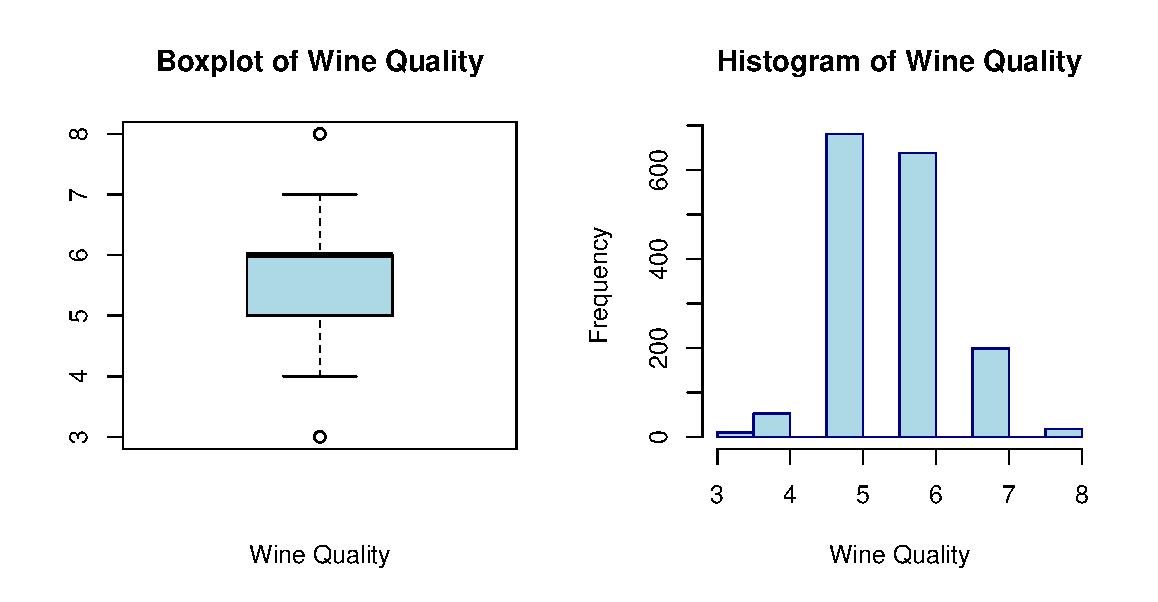
\includegraphics[width=\textwidth]{manuscriptfigure.pdf}
 \caption{A boxplot and a histogram of the wine quality for the samples of Portuguese red wine.}
 \label{fig:wine}
\end{figure}

\section{Methods}
\label{sec:meth}

OVERVIEW PARAGRAPH

\subsection{Classification Methods}
\label{sec:class}

MULTINOMIAL LOGISTIC REGRESSION

In classification, multinomial regression is the name given to the 
logistic regression model that predicts response variable values for 
$K > 2$ classes.  Since it is an extension of logistic regression for 
binary classification, it shares many of the same characteristics.  
Logistic regression models in general are modifications to linear 
regression models that make them fit to return values between 0 and 1.  
Recall that a multiple linear regression model takes the following form:
\begin{equation}
  \label{eq:linreg}
  Y = \beta_0 + \beta_1X_1 + ... + \beta_pX_p + \epsilon.
\end{equation}
In Equation~\eqref{eq:linreg}, we see that there is nothing restricting 
$Y$ from taking values $> 1$ or $< 0$.  This is problematic if we wish 
for our model to predict the probability that the response variable 
falls within a particular class, since probabilities can only take 
values between 0 and 1.  In order to solve this problem, the binary 
classification logistic regression model takes the following form:
\begin{equation}
  \label{eq:logreg}
  p(X) = 
  \frac{e ^ {\beta_0 + \beta_1X_1 + ... + \beta_pX_p}} 
  {1 + e ^ {\beta_0 + \beta_1X_1 + ... + \beta_pX_p}}.
\end{equation}
In Equation~\eqref{eq:logreg}, we see that this problem is essentially 
solved by exponentiation.  The multiple linear regression model is 
placed into the exponent of $e$ to ensure that the numerator and 
denominator will always be positive.  This means that the overall 
model will not return values $< 0$.  Additionally, because the numerator 
will never exceed the denominator, the fraction will always be $\leq 1$.  
Thus, the model outputs values in the desired range for predicting probabilities. 
 Since in binary classification there are only two classes, the output of 
 this model represents the probability that $Y$ will fall into one of the 
 predetermined classes.  The probability that $Y$ will fall into the other 
 class is simply $1 - p(X)$.

 In multinomial logistic regression, however, there are more than 2 classes 
 into which the response variable could fall.  The binary model is generalized 
 to $K > 2$ classes in the following manner:
 \begin{equation}
  \label{eq:multireg}
  Pr( Y = k | X = x ) = 
  \frac{e ^ {\beta_k0 + \beta_k1X_1 + ... + \beta_kpX_p}}
  { \sum_{l = 1} ^ {K}  e ^ {\beta_l0 + \beta_l1X_1 + ... + \beta_lpX_p}},
\end{equation}
where $x$ is a vector of the $p$ predictor values.  In 
Equation~\eqref{eq:multireg}, we see that the numerator is the exponentiated 
linear model for class $k$, while the denominator is the sum of the 
exponentiated linear models for all $K = k$ classes.  It should be noted 
that this is not the only way of generalizing the binary logistic regression 
model to $K >2$ classes.  The model presented in Equation~\eqref{eq:multireg} 
is known as the \textit{softmax} coding \citep{james2021introduction}.  
There are other versions of multinomial regression models, but we will not 
use them and thus not elaborate on them further for this analysis.  

Among the most notable assumptions for the logistic regression model are 
the linear decision boundary and the independence of the predictors used 
in the model \citep{khan2023comparison}.

LINEAR DISCRIMINANT ANALYSIS

QUADRATIC DISCRIMINANT ANALYSIS 

K NEAREST NEIGHBORS

NAIVE BAYES

SUPPORT VECTOR MACHINES

\subsection{Classification Metrics}
\label{sec:metr}

CONFUSION MATRICES

CLASSIFICATION ACCURACY VALUE

AREA UNDER THE ROC CURVE

\section{Results}
\label{sec:resu}

OVERVIEW PARAGRAPH

OPTIONAL: PRESENT CONFUSION MATRICES FOR EACH OF THE METHODS

PRESENT ACC VALUES FOR EACH OF THE METHODS IN COMPARATIVE CHART

PRESENT ROC CURVES FOR EACH OF THE METHODS

PRESENT AUC VALUES FOR EACH OF THE METHODS IN COMPARATIVE CHART

\section{Discussion}
\label{sec:disc}

% What are the main contributions again?

% What are the limitations of this study?

% What are worth pursuing further in the future?

% Watch for prevalence of diabetes \citep{wild2004global}.

\bibliography{references}
\bibliographystyle{chicago}

\end{document}